\documentclass[12pt, titlepage]{article}
\usepackage{float}
\usepackage{tabularx}
\usepackage{graphicx}
\usepackage{paralist}
\usepackage{listings}
\usepackage{booktabs}
\usepackage{hyperref}
\usepackage{amsfonts}
\usepackage{amsmath}
\usepackage{color}
\usepackage{fancyhdr}
\usepackage{geometry}
\geometry{margin = 0.75in}
\hypersetup{
    colorlinks,
    citecolor=blue,
    filecolor=black,
    linkcolor=red,
    urlcolor=blue
}
\usepackage[round]{natbib}

\begin{document}

\title{System Verification and Validation Plan for Digital Twin Forest} 
\author{Team 8, Forest Mirror\\Yichen Jiang\\ Bowen Zhang\\ Jiacheng Wu\\ Junhong Chen\\ Tingyu Shi}
\date{\today}
	
\maketitle

\pagenumbering{roman}

\section{Revision History}

\begin{tabularx}{\textwidth}{p{3cm}p{2cm}X}
\toprule {\bf Date} & {\bf Version} & {\bf Notes}\\
\midrule
October 29th & 1.0 & Initial Document\\
\hline
March 7th & 2.0 & Modify some test cases, finish Design Doc Verification
Plan\\
\hline
April 2 & 3.0 & Final Version\\
\bottomrule
\end{tabularx}

\newpage

\tableofcontents
\listoftables
\listoffigures

\newpage

\section{Symbols, Abbreviations and Acronyms}
The following are some naming conventions and definitions from SRS:
\begin{itemize}
\item LiDAR: Light Detection and Ranging(Scanning Technology)
\item Plot: A square-shaped area in the forest. There are 14 plots in total. 
\item LAI: Leaf Area Index
\item DBH: Diameter at Breast Height
\item Target Forest: Target forest refers to the natural forest located at Turkey
Point in Ontario.
\item Digital Twin Forest: The virtual representation of the target forest.
\item Forest Data: Forest Data include environmental data and tree parameters.
\item Environmental Data:
\begin{itemize}
    \item Humidity
    \item Temperature
    \item Soil Carbon Content
    \item Soil Nitrogen Content
    \item LAI 
\end{itemize}
\item Tree parameters: 
\begin{itemize}
    \item Density
    \item Height
    \item Age
    \item DBH 
\end{itemize}
\item Tree types. There are 7 different types of trees,
the following are the details:
\begin{itemize}
    \item Red Pine
    \item Oak
    \item Birch 
    \item Beech
    \item White Pine
    \item Red Maple
    \item Red Oak
\end{itemize}
\end{itemize}
\newpage

\pagenumbering{arabic}



\section{General Information}
\subsection{Summary}
The software being tested is called \textit{Digital Twin Forest}. 
This is a virtual representation of the target forest. The product 
will provide the following general functions:
\begin{itemize}
\item A virtual representation of the real forest,
allowing monitoring and analyzing from distance.
\item Visualizing important data related to scientific 
research and decision-making.
\item A forest model that can change dynamically 
according to the modification of the data.
\end{itemize}

\subsection{Objectives}

This document will perform as a guide for examining the quality of
our software. The first objective to be accomplished is to make sure
correctness of the software. Testing will allow our team to examine 
all the functions of our product. The software should be executed 
properly, perform as designed, represent the expected data, and
show the model we constructed. The second objective is to examine 
usability. The possible methods might include manual testing by the 
testing team, questionnaires, and user interviews. 

\subsection{Relevant Documentation}
\begin{itemize}
\item \href{https://github.com/wuj187/DigitalTwinCAS/blob/main/docs/SRS/SRS.pdf}{SRS}

\item \href{https://github.com/wuj187/DigitalTwinCAS/blob/main/docs/DevelopmentPlan/DevelopmentPlan.pdf}{Development Plan}

\item \href{https://github.com/wuj187/DigitalTwinCAS/blob/main/docs/Design/Software-Detailed-Design/MIS.pdf}{MIS}

\item \href{https://github.com/wuj187/DigitalTwinCAS/blob/main/docs/Design/Software-Architecture-Design/MG.pdf}{MG}
\end{itemize}

\newpage

\section{Plan}

\subsection{Verification and Validation Team}
\begin{table}[H]
    \centering
    \begin{tabular}{|c|c|}
    \hline
         Team Member  & Roles\\
         \hline
         Yichen Jiang & Test leader\\
         \hline
         Bowen Zhang  & Hardware verification and SRS verification\\
         \hline
         Junhong Chen & Code verification\\
         \hline
         Jiacheng Chen & Code verification\\
         \hline
         Tingyu Shi & SRS verification and Code verification\\
         \hline
         Dr.Gonsamo & Manual testing as user\\
         \hline
         Dr.Gonsamo's lab's members  & Manual testing as users\\
         \hline
         Classmates & Manual testing as users\\
         \hline
    \end{tabular}
    \caption{Team Members and Roles}
\end{table}

\subsection{SRS Verification Plan}
SRS testing refers to the review of the functional and 
non-functional requirements mentioned in the SRS document. In 
general, a SRS checklist will be created to verify if each
requirement has been met. The SRS may be revised by adding or
removing requirements based on new users' needs and constraints.

\subsubsection{Review by Supervisor}
The project is supervised by Dr. Gonsamo and his lab members. Our 
team meets weekly with graduate students in Dr. Gonsamo's lab and 
reviews the progress of the project.
At the end of the semester, our team will have a formal meeting
with Dr. Gonsamo, and the project will be verified to see if it 
accomplishes all his expectations.  Dr. Gonsamo will take the 
project and do a task-based inspection. For example, the 
application will be installed on lab computers, and functions like 
measuring the distance between trees will be tested to see if it has 
an acceptable accuracy.

\subsubsection{Review by Classmates}
Classmates from other groups will be considered users who have no 
training. Non-functional requirements in SRS can be tested by 
these reviewers, and they will provide feedback. For example, it 
is clear that the application is easy to learn if the reviewers 
successfully access the virtual forest in one minute.

\subsubsection{Review by teammates}
Team members are the reviewers who are most familiar with the 
project. The team will
go through the SRS document and carry out both system tests and 
unit tests. 
The SRS checklist will be filled to see if all the functional and
non-functional requirements have been accomplished.

\subsection{Design Verification Plan}
Our design will be continuously improved with the implementation
work heading on the final version. The design documents will be
verified using the following way:
\begin{itemize}
\item Take the feedback from the teaching assistant and peer
reviews 
\item Make sure that design documents are consistent with the 
SRS
\item Make sure that design documents are consistent with the code
(During implementation, we cannot make sure that the actual code 
can follow design documents strictly. Therefore, we also 
need to make sure that design documents are consistent with 
the source code)
\end{itemize}

\subsection{Verification and Validation Plan Verification Plan}
The verification and validation plan verification plan aims at 
documenting how this verification and validation plan will be 
verified. The VnV plan will be reviewed by classmates from other 
groups and TAs, and we will collect feedback and questions from 
them. The VnV plan will also be verified by the ForestMirror team 
when team members perform tests for the functional and 
non-functional requirements mentioned in SRS, and any 
modifications of the testing plans will be recorded. 

\subsection{Implementation Verification Plan}
Implementation verification refers to the high-quality code of the 
application. Code testing is mentioned in the system test 
description of this document, especially in the tests for
nonfunctional requirements. For example, dynamic testing will be done
for performance requirements, and the team will perform individual code
walkthroughs. The team will follow the module guide and the traceability matrix to see
if the system follows low coupling and high cohesion principles, and another team member will help him/her do the
verification.
If the test fails, the code needs to be revised
before committing.\\
\noindent
Besides that, we will use static testing to ensure the code and documents are following good quality and our design. During the development, we will contact our stakeholders to make sure we are making the right products.

\subsection{Automated Testing and Verification Tools}

Automated testing tools will not be used in our project. As the team uses the visual studio as the IDE and the scripts will be automatically compiled. Unity will respond to the modification as a system. Therefore, all the tests will be done manually in Unity.

\subsection{Software Validation Plan}
Software validation is to guarantee SRS captures the right requirements.  As a
Meteorologist, Dr. Gonsamo, is not only the supervisor of the project but also a
stakeholder. As mentioned in the SRS verification section, Dr. Gonsamo will do a task-based inspection with the team after the Rev 0 demo. The functions of the application will be tested by trying to accomplish a range of tasks just to see if the requirements are necessary.

\newpage

\section{System Test Description}
\subsection{Tests for Functional Requirements}
The system tests about functional requirements
are divided into two subsets. The first subset is about 
testing presentations(what
contents will be presented to users). The second subset is about
testing if users can interact successfully with the product.
According to the SRS document, we have
16 functional requirements in total. The following are the
corresponding requirements within  two subsets
\begin{itemize}
\item Presentation = \{FR1, FR2, FR3, FR7, FR10, FR13, FR14, FR15,
FR16\}
\item Users' interactions with the product = \{FR4, FR5, FR6, 
FR8, FR9, FR11, FR12\}
\end{itemize}

\subsubsection{Presentation}
\begin{enumerate}
%%%%% Test-FR1 %%%%%%%%%%%%%%%%%%%%%%%%%%%%%%%%%
\item{Test-FR1\\}
Control: Manual\\ 

Initial State: The product is just launched and running. The main 
page is presented to users.\\

Input: A click event on \verb|Instruction| button on the main page.\\

Output: The instruction page will open, and instructions about how 
to use the product will be presented on the instruction page.\\

Test Case Derivation: \verb|Instruction| button is designed for 
opening the instruction page that contains instructions. Therefore, 
a click event on \verb|Instruction| button will open the instruction
page.\\
					
How test will be performed: Let testers lunch the software and click
on  \verb|Instruction| button. The instruction page with 
instructions should appear on the  screen. After the instruction 
page has been displayed, testers set the system to the 
initial state(Main page) and retest the \verb|Instruction| button. 
Testers need to repeat this process 10 times.
%%%%%%%%% Test-FR1 End %%%%%%%%%%%%%%%%%%%%%%%%%%%%%%%%%%%%%

%%%%% Test-FR2 %%%%%%%%%%%%%%%%%%%%%%%%%%%%%%%%%
\item{Test-FR2\\}
Control: Manual\\ 

Initial State: The product is just launched and running. The main 
page is presented to users.\\

Input: A click event on \verb|Contact Us| button on the main page.\\

Output: The contact us page will open, and developers' names and
emails should appear on the screen.\\

Test Case Derivation: \verb|Contact Us| button is designed for 
opening the Contact Us page. Therefore, 
a click event on \verb|Contact Us| button will open the Contact 
Us information page.\\
					
How test will be performed: Let testers lunch the software and click
on  \verb|Contact Us| button. The Contact Us information page with 
developers' names and emails should appear on the  screen. 
After the instruction page has been displayed, testers set the 
system to the initial state(Main page) and retest the 
\verb|Contact Us| button. Testers need to repeat this process 10 times.
%%%%%%%%% Test-FR2 End %%%%%%%%%%%%%%%%%%%%%%%%%%%%%%%%%%%%%


%%%%%%%%%%%%%%%%%%%%%%% Test-FR3 %%%%%%%%%%%%%%%%%%%%%%%%%%
\item{Test-FR3\\}
Control: Manual\\ 

Initial State: The product is just launched and running. Main page
is presented to users.\\

Input: A click event on \verb|Start| button on the main page.\\

Output: The full view of forest plot 1 should be displayed. \\

Test Case Derivation: Our system can present forest models of
14 plots and overall forest. The initial forest model presentation
is set to be plot 1. Therefore, after clicking \verb|Start|, 
the forest model of plot 1 should be displayed.\\
					
How test will be performed: Let testers lunch the product and click 
\verb|Start| button 10 times, full view of plot 1 should be 
displayed. After each click, reset the system to the initial 
state.
%%%%%%%%%%%%%%%%%%%% Test-FR3 End %%%%%%%%%%%%%%%%%%%%%%%%%


%%%%%%%%%%%%%%%%%%%%%%% Test-FR7.1 %%%%%%%%%%%%%%%%%%%%%%%%%%
\item{Test-FR7.1\\}
Control: Manual\\ 

Initial State: The forest model is presented to users, and 
environmental data are not displayed.\\

Input: A click event on \verb|Environmental Data| button.\\

Output: Environmental data should appear on the left side of the 
screen.\\

Test Case Derivation: Environmental data are designed to be placed
on the left side of the screen. This can leave the center part 
of the screen to allow users to view the forest model.\\
					
How test will be performed: Let testers click 
\verb|Environmental Data| button 10 times. After each click, testers 
should reset the system to the initial state. Environmental data 
should display on the left side of the screen 10 times.
%%%%%%%%%%%%%%%%%%%% Test-FR7.1 End %%%%%%%%%%%%%%%%%%%%%%%%%

%%%%%%%%%%%%%%%%%%% Test-FR7.2 %%%%%%%%%%%%%%%%%%%%%%%%%%%%%%%
\item{Test-FR7.2\\}
Control: Manual\\ 

Initial State: The forest model is presented to users, and 
tree parameters are not displayed.\\

Input: A click event on \verb|Tree Parameters| button.\\

Output: Tree parameters should appear on the right side of the 
screen.\\

Test Case Derivation: Tree parameters are designed to be placed
on the right side of the screen. This can leave the center part 
of the screen to allow users to view the forest model.\\
					
How test will be performed: Let testers click 
\verb|Tree Parameters| button 10 times. After each click, testers 
should reset the system to the initial state. Tree parameters
should display on the right side of the screen 10 times.
%%%%%%%%%%%%%%% Test-FR7.2 End %%%%%%%%%%%%%%%%%%%%%%%%%%%%%%%

%%%%%%%%%%%%%%% Test-FR10.1 %%%%%%%%%%%%%%%%%%%%%%%%%%%%%%%%%%
\item{Test-FR10.1\\}
Control: Manual\\ 

Initial State: Environmental data are presented.\\

Input: Testers record all the environmental data.\\

Output: N/A\\

Test Case Derivation: Since this test does not have any output, this 
part is not applicable.\\
					
How test will be performed: Let testers observe and record all the 
environmental data. Then testers need to check if the data observed
from the UI are exactly the same as the data stored in the software. 
If the data observed are the same as the data stored in the UI, 
the test passes. Otherwise, the test fails. Testers can check the JSON
files stored \href{https://github.com/tingyushi/DTForest-DS}{here}
as the data to be compared. 
%%%%%%%%%%%%%%% Test-FR10.1 End %%%%%%%%%%%%%%%%%%%%%%%%%%%%%%

%%%%%%%%%%%%%%% Test-FR10.2 %%%%%%%%%%%%%%%%%%%%%%%%%%%%%%%%%%
\item{Test-FR10.2\\}
Control: Manual\\ 

Initial State: Tree Parameters are presented.\\

Input: Testers record all the tree parameters.\\

Output: N/A\\

Test Case Derivation: Since this test does not have any output, this 
part is not applicable.\\
					
How test will be performed: Let testers observe and record all the 
tree parameters. Then testers need to check if the data observed
from the UI are exactly the same as the data stored in the software. 
If the data observed are the same as the data stored in the UI, 
the test passes. Otherwise, the test fails. Testers can check the JSON
files stored \href{https://github.com/tingyushi/DTForest-DS}{here}
as the data to be compared. 
%%%%%%%%%%%%%%% Test-FR10.2 End %%%%%%%%%%%%%%%%%%%%%%%%%%%%%%

%%%%%%%%%%%%%%% Test-FR13 %%%%%%%%%%%%%%%%%%%%%%%%%%%%%%%%%%
\item{Test-FR13\\}
Control: Manual\\ 

Initial State: Forest model is presented.\\

Input: Testers update tree parameters, including tree density, tree
height, and tree DBH.\\

Output: Tree models should change correspondingly according to newly
updated data. For example, if we update the tree height to a larger
value, the tree models should appear higher.\\

Test Case Derivation: Tree model and tree parameter synchronization
means that tree  models should be consistent with the tree parameters.
Therefore, if tree models can change accordingly after  entering 
new tree parameters, we can prove that the synchronization is 
successful.\\
					
How test will be performed: Let testers modify tree parameters for 
all 7 types of trees in 14 plots. After each modification, testers need
to check if the tree models have been updated correctly.
%%%%%%%%%%%%%%% Test-FR13 End %%%%%%%%%%%%%%%%%%%%%%%%%%%%%%

%%%%%%%%%%%%%%% Test-FR14 %%%%%%%%%%%%%%%%%%%%%%%%%%%%%%%%%%
\item{Test-FR14\\}
Control: Manual\\ 

Initial State: Forest model is presented.\\

Input: Testers click on the \verb|seasonal change| button at the top 
center of the screen.\\

Output: 
\begin{itemize}
\item If the current season is summer, all the trees except pine trees
should lose leaves after clicking the \verb|seasonal change| button.
Also, the snow effect should appear.
\item If the current season is winter, all the trees will have leaves 
after clicking the \verb|seasonal change| button. Also, the snow 
effect should disappear.
\end{itemize}

Test Case Derivation: \verb|Seasonal change| button is designed for 
simulating different seasons. Therefore, 
a click event on \verb|seasonal change| button will make the system 
simulate different seasons.\\
					
How test will be performed: Let testers click on \verb|seasonal change|
button 10 times in succession, the summer season and winter season 
should appear 5 times, respectively.
%%%%%%%%%%%%%%% Test-FR14 End %%%%%%%%%%%%%%%%%%%%%%%%%%%%%%

%%%%%%%%%%%%%%% Test-FR15 %%%%%%%%%%%%%%%%%%%%%%%%%%%%%%%%%%
\item{Test-FR15\\}
Control: Manual\\ 

Initial State: Environmental data are displayed.\\

Input: Testers click on the \verb|switch| button located in the 
panel that contains environmental data.\\

Output: A pie chart indicating percentages of different tree 
types should appear on the left side of the screen.\\

Test Case Derivation: \verb|Switch| button is designed for 
displaying the pie chart. Therefore,  a click event on \verb|switch| 
button will visualize the pie chart.\\
					
How test will be performed: Let testers click on \verb|switch|
button 10 times, the pie chart should appear 10 times. After each 
click event, testers need to reset the system to the initial state.
%%%%%%%%%%%%%%% Test-FR15 End %%%%%%%%%%%%%%%%%%%%%%%%%%%%%%

%%%%%%%%%%%%%%% Test-FR16 %%%%%%%%%%%%%%%%%%%%%%%%%%%%%%%%%%
\item{Test-FR16\\}
Control: Manual\\ 

Initial State: The forest model of a plot is loaded and presented.\\

Input: Testers move to the top view of this forest plot.\\

Output: N/A\\

Test Case Derivation: Testers need to verify that tree 
distribution is the same as the satellite pictures provided. \\
					
How test will be performed: Let testers move to the top view of each 
plot and check if the tree distribution is consistent with the 
satellite picture provided. Figure \ref{fig:SP} is a sample satellite picture.
%%%%%%%%%%%%%%% Test-FR16 End %%%%%%%%%%%%%%%%%%%%%%%%%%%%%%

\end{enumerate}


\subsubsection{Users' interactions with the product}
\begin{enumerate}
%%%%%%%%%%%%%%% Test-FR4.1 %%%%%%%%%%%%%%%%%%%%%%%%%%%%%%%%%%
\item{Test-FR4.1\\}
Control: Manual\\ 

Initial State: Environmental data are displayed.\\

Input: A click event on \verb|Environmental Data| button.\\

Output: Environmental data display should disappear from the screen.\\

Test Case Derivation: If environment data can disappear from the 
screen, this proves that data GUI can be minimized.\\
     
How test will be performed: Let testers click 
\verb|Environmental Data| button 10 times when environmental data 
are displayed. Environmental data display should disappear 10 times.
After each click, testers need to reset the system to the initial 
state.
%%%%%%%%%%%%%%% Test-FR4.1 End %%%%%%%%%%%%%%%%%%%%%%%%%%%%%%

%%%%%%%%%%%%%%% Test-FR4.2 %%%%%%%%%%%%%%%%%%%%%%%%%%%%%%%%%%
\item{Test-FR4.2\\}
Control: Manual\\ 

Initial State: Tree parameters are displayed.\\

Input: A click event on \verb|Tree Parameters| button.\\

Output: Tree parameters display should disappear from the screen.\\

Test Case Derivation: If tree parameters can disappear from the 
screen, this proves that data GUI can be minimized.\\
     
How test will be performed: Let testers click 
\verb|Tree Parameters| button 10 times when tree parameters 
are displayed. Tree parameters display should disappear 10 times.
After each click, testers need to reset the system to the initial 
state.
%%%%%%%%%%%%%%% Test-FR4.2 End %%%%%%%%%%%%%%%%%%%%%%%%%%%%%%

%%%%%%%%%%%%%%% Test-FR5 %%%%%%%%%%%%%%%%%%%%%%%%%%%%%%%%%%
\item{Test-FR5\\}
Control: Manual\\ 

Initial State: Forest model is loaded and presented.\\

Input: A click event on \verb|Environmental Data| button.\\

Output: The panel to present environmental data should appear on the left side 
of the screen.\\

Test Case Derivation: If clicking on \verb|Environmental Data| button can 
visualize environmental data, we can prove that our system has provided 
a way to visualize environmental data.\\
					
How test will be performed:  Let testers click \verb|Environmental Data| button
10 times, environmental data should be displayed 10 times. After 
each click event, testers need to reset the system to the initial state.
%%%%%%%%%%%%%%% Test-FR5 End %%%%%%%%%%%%%%%%%%%%%%%%%%%%%%

%%%%%%%%%%%%%%% Test-FR6 %%%%%%%%%%%%%%%%%%%%%%%%%%%%%%%%%%
\item{Test-FR6\\}
Control: Manual\\ 

Initial State: Forest model is loaded and presented.\\

Input: A click event on \verb|Tree Parameters| button.\\

Output: The panel to present tree parameters should appear on the 
right side of the screen.\\

Test Case Derivation: If clicking on \verb|Tree Parameters| 
button can  visualize tree parameters, we can prove that our 
system has provided a way to visualize .\\
					
How test will be performed:  Let testers click 
\verb|Tree parameters| button
10 times, tree parameters should be displayed 10 times. After 
each click event, testers need to reset the system to the initial state.
%%%%%%%%%%%%%%% Test-FR6 End %%%%%%%%%%%%%%%%%%%%%%%%%%%%%%


%%%%%%%%%%%%%%% Test-FR8 %%%%%%%%%%%%%%%%%%%%%%%%%%%%%%%%%%
\item{Test-FR8\\}
Control: Manual\\ 

Initial State: Forest model is loaded and presented.\\

Input: Testers press \verb|WASD| keys.\\

Output: 
\begin{itemize}
\item Users move forward after pressing \verb|W| key.
\item Users move backward after press \verb|S| key.
\item Users move left after pressing \verb|A| key.
\item Users move right after pressing \verb|D| key.
\end{itemize}

Test Case Derivation: In Unity, we can program \verb|WASD| keys
so that they can control the movement of the camera. If the 
camera can move around in the forest, users can move in the 
forest equivalently.\\
					
How test will be performed:
\begin{itemize}
\item Let testers press \verb|A| key 5 times in succession 
and each key press should last 2 seconds.  The user's point of 
view should move left after each key press.

\item Let testers press \verb|D| key 5 times in 
succession, and each key press should last 2 seconds. The user's
point of view  should move right after each key press.

\item Let testers press \verb|W| key 5 times in 
succession, and each key press should last 2 seconds. The user's
point of view  should move forward after each key press.

\item Let testers press \verb|S| key 5 times in 
succession, and each key press should last 2 seconds. The user's
point of view  should move backward after each key press.
\end{itemize}
%%%%%%%%%%%%%%% Test-FR8 End %%%%%%%%%%%%%%%%%%%%%%%%%%%%%%

%%%%%%%%%%%%%%% Test-FR9 %%%%%%%%%%%%%%%%%%%%%%%%%%%%%%%%%%
\item{Test-FR9\\}
Control: Manual\\ 

Initial State: The forest model is presented on the screen.\\

Input: Users move the mouse in 4 different directions, which are
left, right, forward, and backward.\\

Output:
\begin{itemize}
    \item Move the mouse forward: The user's first point of view should rotate up.
    \item Move the mouse backward: The user's first point of view should rotate 
    down.
    \item Move the mouse left: The user's first point of view should rotate left.
    \item Move the mouse right: The user's first point of view should rotate right.
\end{itemize}

Test Case Derivation: In Unity, the mouse can be programmed to adjust the 
angle of the camera. Therefore,  moving the mouse can change the point of view.\\
					
How test will be performed: \\ The test will be performed in 4 steps:
\begin{enumerate}[1.]
    \item Let testers move the mouse left, the point of view should rotate left.
    \item Let testers move the mouse right, the point of view should rotate right.
    \item Let testers move the mouse forward, the point of view should rotate up.
    \item Let testers move the mouse backward, the point of view should rotate down.
\end{enumerate}
%%%%%%%%%%%%%%% Test-FR9 End %%%%%%%%%%%%%%%%%%%%%%%%%%%%%%

%%%%%%%%%%%%%%% Test-FR11 %%%%%%%%%%%%%%%%%%%%%%%%%%%%%%%%%%
\item{Test-FR11\\}
Control: Manual\\ 

Initial State: Main page is presented to users.\\

Input: A click event on \verb|Quit| button.\\

Output: Software should close.\\

Test Case Derivation: \verb|Quit| button is designed for quitting
the software, so clicking \verb|Quit| button quit the software.\\
					
How test will be performed:  Let testers click \verb|Quit| button 
located in the main page. After clicking \verb|Quit| button, the
software should close.
%%%%%%%%%%%%%%% Test-FR11 End %%%%%%%%%%%%%%%%%%%%%%%%%%%%%%

%%%%%%%%%%%%%%% Test-FR12 %%%%%%%%%%%%%%%%%%%%%%%%%%%%%%%%%%
\item{Test-FR12\\}
Control: Manual\\ 

Initial State: Update data page is presented.\\

Input: Testers enter new data in the input box and click \verb|Update| Button\\

Output: A text should pop up indicating if the update was successful.\\

Test Case Derivation: N/A.\\
					
How test will be performed: \\ The test will be performed in the following ways:
\begin{enumerate}[1.]
\item Testers select a plot.
\item Testers select updating environmental data or tree parameters. (If testers
choose to update tree parameters, testers also need to choose a tree type.)
\item Testers select the data type.
\item Testers enter the new data.
\item Testers press \verb|Update| button.
\item Testers should enter the forest model to check if the newly updated data can 
appear in the environmental data display or tree parameters display. 
\item Repeat the above steps for all 14 plots and 7 tree types.
\end{enumerate}
%%%%%%%%%%%%%%% Test-FR12 End %%%%%%%%%%%%%%%%%%%%%%%%%%%%%%
\end{enumerate}


\subsection{Tests for Nonfunctional Requirements}

\subsubsection{Look and Feel Requirement testing}

\begin{enumerate}

\item{Test-NFR-LF1.1\\}
Type: Static\\

How test will be performed: Testers conduct interviews with random people to gather feedback by providing the questionnaire in the Appendix and expect that over 80 percent of the users will agree that the forest model is close to the real forest.\\

Expected result: Over 80 percent of the users choose A or B in the first question in the questionnaire.

\item{Test-NFR-LF2.1\\}

Type: Static\\

How test will be performed: Testers compared the forest data stored in the software with physical measurements and then calculated the relative errors of the data.\\

Expected result: All the forest data have errors less than 0.1 compared to the actual data provided by our client. 

\item{Test-NFR-LF2.2\\}

Type: Static\\

How test will be performed: Testers conduct interviews with random people to gather feedback by providing the questionnaire in the Appendix and expect that over 80 percent of the users will answer that the system looks professional.\\

Expected result: Over 80 percent of the users choose A or B in the second question in the questionnaire.

\subsubsection{Usability and Humanity Requirements testing}
\item{Test-NFR-UH1.1\\}

Type: Static\\

How test will be performed: Testers conduct interviews with random people to gather feedback by providing the questionnaire in the Appendix, and expect that over 80 percent of the users will answer that the instructions are easy to understand. \\

Expected result: Over 80 percent of the users choose A or B in the third question in the questionnaire.

\item{Test-NFR-UH2.1\\}

Type: Manual\\

Initial State: The system is launched\\

Input: Testers inspect all the texts on every UI component in the software \\

Output: All of the texts are in English\\

How test will be performed: Testers launch the software and inspect all the components containing texts in the software.

\item{Test-NFR-UH3.1\\}

Type: Manual\\

Initial State: The system is launched and it is on the main page\\

Input: A click event is made on the instructions option\\

Output: Instructions are displayed after the event\\

How test will be performed: Testers click on the instruction option, observe the response and expect that instructions will be displayed on the screen. \\

\item{Test-NFR-UH4.1\\}

Type: Static\\

How test will be performed: Testers conduct interviews with random adults to gather feedback by providing the questionnaire in the Appendix and expect that over 80 percent of the users will answer that they notice and understand all icons.\\

Expected result: Over 80 percent of the users choose A or B in the fourth question in the questionnaire.

\item{Test-NFR-UH4.2\\}

Type: Static\\

How test will be performed: Testers conduct interviews with random adults to gather feedback by providing the questionnaire in the Appendix and expect that over 80 percent of the users will answer that they think the icons used in the software are appealing.\\

Expected result: Over 80 percent of the users choose A or B in the fifth question in the questionnaire.

\item{Test-NFR-UH5.1\\}

Type: Manual\\

Initial State: The system is launched\\

Input: Input from mouse and keyboard from users\\

Output: All interactive components, such as buttons and sliding bars, can be controlled by both mouse and keyboard\\

How test will be performed: Testers launch the software and try to access all the interactive components in the software using a mouse and keyboard. Testers should be able to complete all the actions without any trouble.

\item{Test-NFR-UH5.2\\}

Type: Static\\

How test will be performed: Testers conduct interviews with random adults to gather feedback by providing the questionnaire in the Appendix. We expect that over 80 percent of the users will answer that they can learn how to use the system within half an hour.\\

Expected result: Over 80 percent of the users choose A or B in the sixth question in the questionnaire.

\subsubsection{Performance Requirements}
\item{Test-NFR-PR1.1\\}

Type: Manual\\

Initial State: The system is launched\\

Input: Input from mouse or keyboard to make an action in the application\\

Output: The system responds to all mouse or keyboard inputs within 2 seconds\\

How test will be performed: Testers launch the system and test its responsiveness by performing actions such as clicking the start button. The system should respond to any request within 2 seconds.

\item{Test-NFR-PR1.2\\}

Type: Manual\\

Initial State: The system is launched and on the forest page\\

Input: None\\

Output: The system is running at over 30 FPS for 90 percent of the time\\

How test will be performed: Testers record FPS and time. The system should run at over 30 FPS for 90 percent of the time on the forest page.

\item{Test-NFR-PR1.3\\}

Type: Manual\\

Initial State: The system is launched and on the main page\\

Input: A click event is triggered on the start option\\

Output: The system loads all the models within 10 seconds\\

How test will be performed: Testers launch the system and click the start option. They should wait for the models to appear in less than 10 seconds.

\item{Test-NFR-PR3.1\\}

Type: Static\\

How the test will be performed: Testers record all the forest data in the system and compare it to the physical measurements, and then calculate the relative errors of the data\\

Expected result: All the forest data have relative errors of less than 0.1.

\item{Test-NFR-PR4.1\\}

Type: Manual\\

Initial State: The system is not launched\\

Input: Testers give inputs to open the system\\

Output: The system launches successfully 100 percent of the time\\

How the test will be performed: Testers launch the system and observe the system. The system should open successfully 100 percent of the time.

\item{Test-NFR-PR4.2\\}

Type: Manual\\

Initial State: The system is launched\\

Input: Screen recording to record the system\\

Output: The system is working all the time for 24 hours \\

How the test will be performed: Testers launch the software in the background for 24 hours and expect that the software will not crash within the duration.

\item{Test-NFR-PR5.1\\}

Type: Manual\\

Initial State: The system is launched without an internet connection\\

Input: Input from the mouse and the keyboard

Output: The response of the system to the mouse and keyboard inputs. \\

How the test will be performed: Testers open the system without an internet connection, then click all the buttons in the system, press the keyboard keys, and move the mouse on the forest page. All the buttons should respond correctly, and the system should give the correct response to the keyboard and the mouse inputs. 


\item{Test-NFR-PR6.1\\}

Type: Static\\

How the test will be performed: Testers will assess the size of the system after the system is implemented.\\

Expected result: The size of the software is less than 10 GB.

\subsubsection{Operational and Environmental Requirements}
\item{Test-NFR-OE1.1\\}

Type: Manual\\

Initial State: The system is launched on desktops and laptops\\

Input: Inputs of the keyboard and the mouse\\

Output: The system operates normally on desktops and laptops\\

How the test will be performed: Testers will run the system on desktops and laptops, then click all the buttons in the system, press the keyboard keys, and move the mouse on the forest page. All the buttons should respond correctly, and the system should give the correct response to the keyboard and the mouse inputs. 

\item{Test-NFR-OE1.2\\}

Type: Manual\\

Initial State: The system is launched\\

Input: Input from mouse and keyboard from users\\

Output: All tasks are accomplished normally with mouse and keyboard\\

How the test will be performed: Testers open the software, then click all the buttons in the system, press the keyboard keys, and move the mouse on the forest page. Testers should end up finishing all the actions without any trouble, and all the buttons should respond correctly, and the system should give the correct response to the keyboard and the mouse inputs. 

\item{Test-NFR-OE2.1\\}

Type: Manual\\

Initial State: The system is launched on Windows 10 and MacOS 12 or later version\\

Input:  Input from mouse and keyboard from users\\

Output: The system is running normally\\

How the test will be performed: The testers click all the buttons in the system, press the keyboard keys, and move the cursor on the forest page on Windows 10 or later version or MacOS 12 or later version. The system should run normally, all the buttons should respond correctly, and the system should respond correctly to the keyboard and the mouse inputs without breaking down.

\item{Test-NFR-OE3.1\\}

Type: Static\\

Initial State: Testers open the link of the application on GitHub

Input: Click on the download button.

Output: The application is downloaded to testers' computers.

Expected result: The system is downloaded, installed, and runs without any errors and bugs.

How the test will be performed: Testers try to download and install the application from GitHub and observe the process to see if it operates normally.

\item{Test-NFR-OE4.1\\}

Type: Static\\

Initial State: Git commit history of this application\\

Output: Some monthly updates

Expected result: There are some monthly updates in the git commit history

How the test will be performed: Testers check the git commit history and see if there are monthly updates.

\item{Test-NFR-OE4.2\\}

Type: Static\\

Initial State: New versions of the application has been released

Output: Test report of the existing functions

Expected result: Every test case should be passed

How the test will be performed: Testers perform tests on the existing functions after each update and expect that all the tests should pass.

\subsubsection{Maintenance and Support Requirements Testing}

\item{Test-NFR-MS1.1\\}

Type: Static.\\

How the test will be performed: Testers check the documentation of the product to see if the new features, functions, and any modifications are added to the documentation or not.\\

Expected result: new features and functions and modifications should be on the documentation.

\item{Test-NFR-MS1.2\\}

Type: Static.\\

How the test will be performed: Testers read the documentation of the product to see if the documentation specifies the functions clearly.\\

Expected result: All functions on the documents are clearly documented.

\item{Test-NFR-MS1.3\\} 

Type: Manual\\

Initial State: A bug is found in the program.\\

Input: GitHub commit history\\

Output: The bug is fixed in three days.\\

How the test will be performed: Record the time from the bug occurs to the time when the bug is fixed. Measure the time to see if it is within three days. 

\item{Test-NFR-MS2.1\\}

Type: Manual\\

Initial State: Testers open the instruction page and try to find the contact method.\\

Input: Testers use the contact method to contact the developers.\\

Output: Testers can contact the developer and be able to give feedback to them.\\

How the test will be performed: Testers first look for the contact method on the contact page, then use the contact method to contact the developers to see if they can contact the developers successfully or not.  

\item{Test-NFR-MS3.1\\}

Type: Manual\\

Initial State: None\\

Input: Testers launch the application on different operating systems.\\

Output: The application can run on at least one operating system.\\

How the test will be performed: Testers try to launch the application on different operating systems to see if it can be run successfully on a system or not.  

\item{Test-NFR-MS3.2\\}

Type: Manual\\

Initial State: None\\

Input: Testers run the application on the device located indoors and outdoors.\\

Output: The application can run on both indoor and outdoor devices.\\

How the test will be performed: Testers try to launch the application on the devices located indoors and outdoors respectively to see if the application can be used both indoors and outdoors or not.  


\subsubsection{Security Requirements Testing}

\item{Test-NFR-SR1.1\\}

Type: Static.\\

How the test will be performed: Testers try to find and download the product from GitHub and any other website .\\

Expected result: Testers can not download the product in other websites other than GitHub.

\item{Test-NFR-SR1.2\\}

Type: static.\\

How test will be performed: Testers try to update the data of trees and forests via the interface and anywhere else to see if they can update the data successfully or not.\\

Expected result: The testers can only update the data from the specific interface provided by developers.


\item{Test-NFR-SR2.1\\}

Type: Manual\\

Initial State: The scanning result of the computer security application is normal. \\

Input: 100 Errors injected into our software.\\

Output: The scan results of the computer security application are still normal.\\

How the test will be performed: Testers inject 100 errors on purpose in our application and see if the scan results of the computer security application will detect the errors in the computer system or not.

\item{Test-NFR-SR2.2\\}

Type: Manual\\

Initial State: The application is running and behaving properly\\

Input: The use of software for a long time and the constant interactions between the testers and the software.\\

Output: The application will be running in a normal way.\\

How the test will be performed: Testers use the software and perform some complicated tasks such as zooming in and zooming out for a long time to see if the application will crash or not.

\item{Test-NFR-SR2.3\\}

Type: Manual\\

Initial State:The system is in \verb|Update Data| page.\\

Input: Some invalid data.\\

Output: Fail to update the data. And a warning message pops up indicating an invalid update operation.\\

How the test will be performed: Testers input some invalid data in the \verb|Update Data| page. The product should pop up a warning message to indicate invalid input and reject the update request.\\



\item{Test-NFR-SR2.4\\}

Type: Manual\\

Initial State: \verb|Update Data| page is displayed.\\

Input: Update new data into the product. Reach the data just updated in the display.\\

Output: Data displayed matches the data just updated.\\

How the test will be performed: Testers manually update some data into the product, take records, and compare the update with he data currently displayed. The data should be consistent with the data just updated.

\item{Test-NFR-SR2.5\\}

Type: Manual\\

How the test will be performed: Testers manually compare the GUI and data files. Each data should have one unique position to display in the GUI and each GUI should correspond to unique data. 

Expected result: The product shows a one-to-one mapping relationship between data and GUI. 



\item{Test-NFR-SR3.1\\}

Type: Static\\

How the test will be performed: Referring to the feedback of the questionnaire we provided in the Appendix, all of the users answered the product did not ask them to provide their personal information.

Expected result: All the users choose B in the ninth question in the questionnaire.

\item{Test-NFR-SR3.2\\}

Type: Static\\

How the test will be performed: Referring to the feedback of the questionnaire we provided in the Appendix, all of the users answered they didn't receive notifications from the application after they turned off the notification in the application.\\

Expected result: All the users choose B in the seventh question in the questionnaire.\\


\subsubsection{Cultural and Political Requirements Testing}

\item{Test-NFR-CP1.1\\}

Type: Static\\

How the test will be performed: Referring to the feedback of the questionnaire we provided in the Appendix, all the users answered that the contents of the product are not offensive to them.\\

Expected result: All of the users chose B for the eighth question in the questionnaire.


\subsubsection{Legal Requirements Testing}

\item{Test-NFR-LR2.1\\}

Type: Static.\\

How the test will be performed: Testers ask the users if any part appears lawfully unreasonable when spreading the questionnaires.\\

Expected result: A typical citizen should not notice any part lawful unreasonable. 
\end{enumerate}

\newpage

\subsection{Traceability Between Test Cases and Requirements}
\begin{table}[H]
    \centering
    \begin{tabular}{|c|c|}
    \hline
    Function Requirement     &  Test Case ID\\
    \hline
    FR1     & Test-FR1\\
    \hline
    FR2 & Test-FR2\\
    \hline
    FR3 & Test-FR3\\
    \hline
     FR4 & Test-FR4.1, Test-FR4.2\\
    \hline
     FR5 & Test-FR5\\
    \hline
     FR6 & Test-FR6\\
    \hline
     FR7 & Test-FR7.1, Test-FR7.2\\
    \hline
     FR8 & Test-FR8\\
    \hline
     FR9 & Test-FR9\\
    \hline
     FR10 & Test-FR10.1, Test-FR10.2\\
    \hline
     FR11 & Test-FR11\\
    \hline 
     FR12 & Test-FR12\\
    \hline
    FR13 & Test-FR13.1\\
    \hline
    FR14 & Test-FR14\\
    \hline
    FR15 & Test-FR15\\
    \hline
    FR16 & Test-FR16\\
    \hline
    \end{tabular}
    \caption{Traceability between Functional Requirements and Tests}
\end{table}


\begin{table}[H]
    \centering
    \begin{tabular}{|c|c|}
    \hline
    Non-functional Requirement & Test Case ID\\
    \hline
    NFR-LF1.1 & Test-NFR-LF1.1\\
    \hline
    NFR-LF2.1 & Test-NFR-LF2.1\\
    \hline
    NFR-LF2.2 & Test-NFR-LF2.2\\
    \hline
    NFR-UH1.1 & Test-NFR-UH1.1\\
    \hline
    NFR-UH2.1 & Test-NFR-UH2.1\\
    \hline
    NFR-UH3.1 & Test-NFR-UH3.1\\
    \hline
    NFR-UH4.1 & Test-NFR-UH4.1\\
    \hline
    NFR-UH4.2 & Test-NFR-UH4.2\\
    \hline
    NFR-UH5.1 & Test-NFR-UH5.1\\
    \hline
    NFR-UH5.2 & Test-NFR-UH5.2\\
    \hline
    NFR-PR1.1 & Test-NFR-PR1.1\\
    \hline
    NFR-PR1.2 & Test-NFR-PR1.2\\
    \hline
    NFR-PR1.3 & Test-NFR-PR1.3\\
    \hline
    NFR-PR3.1 & Test-NFR-PR3.1\\
    \hline
    NFR-PR4.1 & Test-NFR-PR4.1\\
    \hline
    NFR-PR4.2 & Test-NFR-PR4.2\\
    \hline
    NFR-PR5.1 & Test-NFR-PR5.1\\
    \hline
    NFR-PR6.1 & Test-NFR-PR6.1\\
    \hline
    \end{tabular}
    \caption{Traceability between Non-Functional Requirements and Tests Part 1}
\end{table}


\begin{table}[H]
    \centering
    \begin{tabular}{|c|c|}
    \hline
    Non-functional Requirement & Test Case ID\\
    \hline
    NFR-OE1.1 & Test-NFR-OE1.1\\
    \hline
    NFR-OE1.2 & Test-NFR-OE1.2\\
    \hline
    NFR-OE2.1 & Test-NFR-OE2.1\\
    \hline
    NFR-OE3.1 & Test-NFR-OE3.1\\
    \hline
    NFR-OE4.1 & Test-NFR-OE4.1\\
    \hline
    NFR-OE4.2 & Test-NFR-OE4.2\\
    \hline
    NFR-MS1.1 & Test-NFR-MS1.1\\
    \hline
    NFR-MS1.2 & Test-NFR-MS1.2\\
    \hline
    NFR-MS1.3 & Test-NFR-MS1.3\\
    \hline
    NFR-MS2.1 & Test-NFR-MS2.1\\
    \hline
    NFR-MS3.1 & Test-NFR-MS3.1\\
    \hline
    NFR-MS3.2 & Test-NFR-MS3.2\\
    \hline
    NFR-SR1.1 & Test-NFR-SR1.1\\
    \hline
    NFR-SR1.2 & Test-NFR-SR1.2\\
    \hline
    NFR-SR2.1 & Test-NFR-SR2.1\\
    \hline
    NFR-SR2.2 & Test-NFR-SR2.2\\
    \hline
    NFR-SR2.3 & Test-NFR-SR2.3\\
    \hline
    NFR-SR2.4 & Test-NFR-SR2.4\&2.6\\
    \hline
    NFR-SR2.5 & Test-NFR-SR2.5\\
    \hline
    NFR-SR3.1 & Test-NFR-SR3.1\\
    \hline
    NFR-SR3.2 & Test-NFR-SR3.2\\
    \hline
    NFR-CP1.1 & Test-NFR-CP1.1\\
    \hline
    NFR-LR2.1 & Test-NFR-LR2.1\\
    \hline
    \end{tabular}
    \caption{Traceability between Non-Functional Requirements and Tests Part 2}
\end{table}

\newpage

\section{Unit Test Description}
Unit testing does not accommodate Unity's workflow. Each script
is  automatically compiled by Unity. If the team wants to test a 
particular module, they still have to run the whole system and
check the Unity console. As a result, all unit testing are
included in the system testing. 

\newpage

\section{Appendix}

This is where you can place additional information.

\subsection{Symbolic Parameters}
N/A

\subsection{Usability Survey Questionnaire}
\centering

\begin{enumerate}
    \item The virtual forest is lifelike compared to the real forest
\begin{enumerate}[a.]
        \item Strongly Agree
        \item Agree
        \item Neutral
        \item Disagree
        \item Strongly Disagree
    \end{enumerate}
    \item Digital Twin Forest is professional
    \begin{enumerate}[a.]
        \item Strongly Agree
        \item Agree
        \item Neutral
        \item Disagree
        \item Strongly Disagree
    \end{enumerate}
    \item The product instructions are easy to understand
    \begin{enumerate}[a.]
        \item Strongly Agree
        \item Agree
        \item Neutral
        \item Disagree
        \item Strongly Disagree
        \end{enumerate}
    \item You noticed the highlighted icons and understand their functionalities
        \begin{enumerate}[a.]
            \item Strongly Agree
            \item Agree
            \item Neutral
            \item Disagree
            \item Strongly Disagree
            \end{enumerate}
    \item The icons on the user interface are appealing to you
        \begin{enumerate}[a.]
            \item Strongly Agree
            \item Agree
            \item Neutral
            \item Disagree
            \item Strongly Disagree
            \end{enumerate}

    \item How much time did you spend learning to use our product?
        \begin{enumerate}[a.]
            \item Strongly Agree
            \item Agree
            \item Neutral
            \item Disagree
            \item Strongly Disagree
            \end{enumerate}

    \item Did you receive any notification from the application after you disabled the notifications on the setting page of the application?
        \begin{enumerate}[a.]
            \item Yes
            \item No
            \end{enumerate}

    \item Are there any contents like texts, icons and modules in the products that you think are offensive to you?
        \begin{enumerate}[a.]
            \item Yes
            \item No
            \end{enumerate}

    \item Did your product ask you to provide your personal information?
        \begin{enumerate}[a.]
            \item Yes
            \item No
            \end{enumerate}
\end{enumerate}

\newpage

\subsection{Pictures}
The following is a sample turn page button:
\begin{figure}[H]
    \centering
    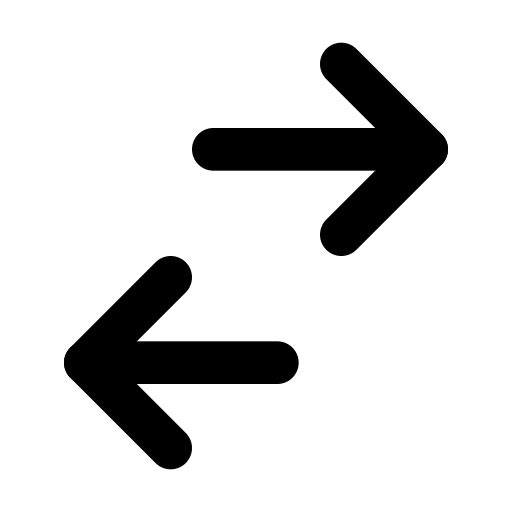
\includegraphics[scale = 0.5]{VnV_Pictures/turnpage_icon.png}
    \caption{Turn Page Button}
\end{figure}

\noindent The following is a sample minimize button:
\begin{figure}[H]
    \centering
    
\includegraphics[scale = 0.5]{VnV_Pictures/tree_parameter.png}
    \caption{Show/Minimize Tree Parameter Data Button}
\end{figure}

\begin{figure}[H]
    \centering
    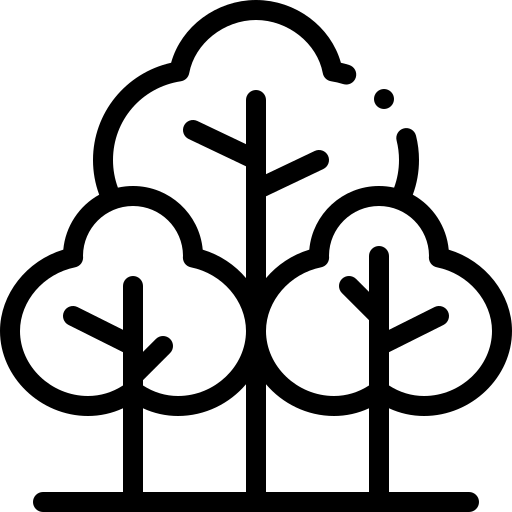
\includegraphics[scale = 0.5]{VnV_Pictures/environmental_data.png}
    \caption{Show/Minimize Environmental Data Button}
\end{figure}

\begin{figure}[H]
    \centering
    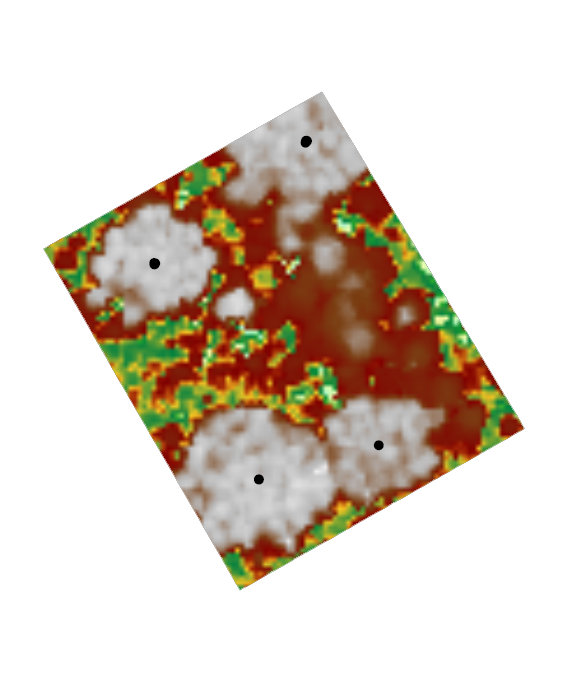
\includegraphics{VnV_Pictures/Satallite-Pic.png}
    \caption{Sample Satellite Picture}
    \label{fig:SP}
\end{figure}

\newpage


\newpage{}
\section*{Appendix --- Reflection}

The information in this section will be used to evaluate the team members on the
graduate attribute of Lifelong Learning.  Please answer the following questions:

\begin{enumerate}
  \item What knowledge and skills will the team collectively need to acquire to
  successfully complete the verification and validation of your project?
  Examples of possible knowledge and skills include dynamic testing knowledge,
  static testing knowledge, specific tool usage etc.  You should look to
  identify at least one item for each team member.
  \item For each of the knowledge areas and skills identified in the previous
  question, what are at least two approaches to acquiring the knowledge or
  mastering the skill?  Of the identified approaches, which will each team
  member pursue, and why did they make this choice?
\end{enumerate}

The knowledge and skills the team need to acquire to complete the verification and validation of our project are listed below:
\begin{itemize}
    \item dynamic testing knowledge
    \item static testing knowledge
    \item automatic and manual testing knowledge
    \item the use of Unity
    \item design of questionnaire and user interview
\end{itemize}

Jiacheng is responsible for dynamic testing knowledge. The possible approaches to acquire it include online tutorials and the experience of the mandatory testing course we took last semester. He decided to pursue this knowledge because it is essential for the validation of the product, and the correctness has to be proved in the process of execution. Furthermore, he is familiar with dynamic testing knowledge.\\

Tingyu is responsible for static testing knowledge. Possible approaches to acquire this kind of knowledge could be the experience of a testing course we took, searching online, discussing in the group and talking to experts. Static testing is significant in the verification process, and it would include technical or informal review, inspection, walkthrough, static code review, etc. As Tingyu is also responsible for organizing regular meetings and taking the script, he would love to study static testing knowledge and put static testing into our meetings as a part of the discussion. He would control and manage the process of static testing.\\

Yichen is responsible for automatic and manual testing knowledge. Knowledge about automatic and manual testing can be gained from the online materials, experience in the testing course, and more. The knowledge of automatic testing will mainly apply to parametric modelling and data storage. And manual testing will be used on the other part, as our product relies on the user interface, and we have to check the overall results manually. Yichen decided to pursue this kind of knowledge because she will take care of the overall effect of the user interface and make modifications along with the testing results. \\

Bowen is responsible for the use of Unity. The possible methods of gaining knowledge of Unity include online tutorials, experience from past courses, and talking to experts. Bowen will work as the main developer for the modelling part and has one year of CO-OP experience working on Unity, and that is why he will pursue this skill.\\

Junhong is responsible for the design of the questionnaire and user interview. The possible approaches to gaining this skill include learning in human-computer interaction class, searching online, and learning about successful cases we can find. This skill is essential because we would love to know how the user feels using our product to get a full view of the usability and user experience. Moreover, this can only be achieved by asking our users. Junhong decided to pursue this one because he already deeply understands this skill and has performed many independent projects with questionnaires. 
\end{document}